\documentclass[border=10pt]{standalone}
\usepackage{tikz}
\definecolor{myred}{RGB}{190,60,45}
\definecolor{mygreen}{RGB}{30,130,40}
\begin{document}
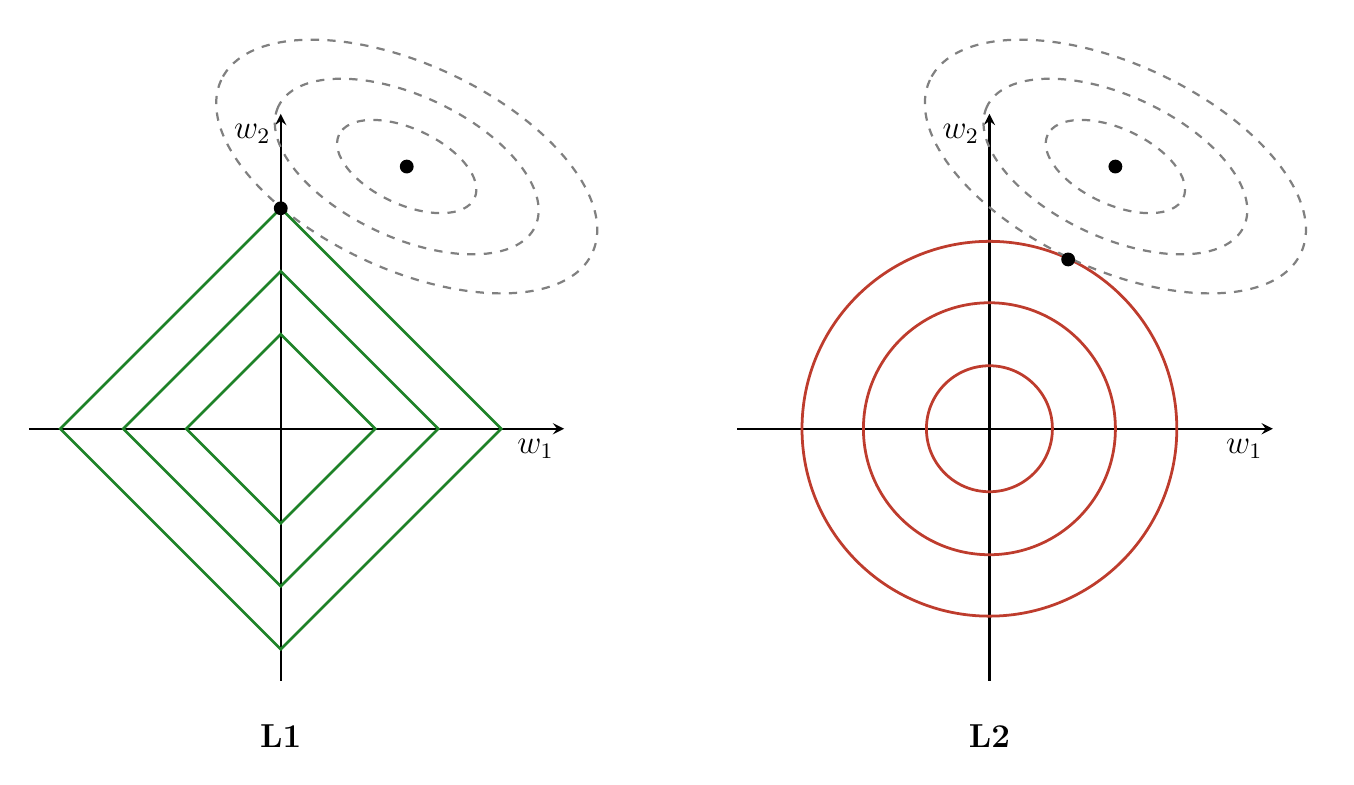
\begin{tikzpicture}[>=stealth, line width=0.8pt, font=\large]

  % ===== 左：L1（菱形），外圈损失等高线精确穿过轴顶点 =====
  \begin{scope}[xshift=0cm]
    \draw[->] (-3.2,0) -- (3.6,0) node[below left] {$w_1$};
    \draw[->] (0,-3.2) -- (0,4.0) node[below left] {$w_2$};
    \begin{scope}[shift={(1.6,3.33)}, rotate=155]
      \foreach \a/\b in {0.95/0.48, 1.8/0.9, 2.6/1.3}
        \draw[gray, dashed] (0,0) ellipse (\a cm and \b cm);
    \end{scope}
    \fill[black] (1.6,3.33) circle (2.5pt);                 % 真实最小值
    \foreach \c in {1.2,2.0,2.8}
      \draw[mygreen, line width=1pt] (0,\c) -- (\c,0) -- (0,-\c) -- (-\c,0) -- cycle;
    \fill[black] (0,2.8) circle (2.5pt);                   % 正则后解 = 顶点 = 接触点
    \node[font=\large\bfseries] at (0,-3.9) {L1};
  \end{scope}

  % ===== 右：L2（圆），圆与损失等高线真相切 =====
  \begin{scope}[xshift=9cm]
    \draw[->] (-3.2,0) -- (3.6,0) node[below left] {$w_1$};
    \draw[->] (0,-3.2) -- (0,4.0) node[below left] {$w_2$};
    \foreach \r in {0.8,1.6,2.38}
      \draw[myred, line width=1pt] (0,0) circle (\r cm);
    % 椭圆短轴沿 OP 方向、短轴顶点=切点 P → 数学相切
    \begin{scope}[shift={(1.6,3.33)}, rotate=155]
      \foreach \a/\b in {0.95/0.48, 1.8/0.9, 2.6/1.3}
        \draw[gray, dashed] (0,0) ellipse (\a cm and \b cm);
    \end{scope}
    \fill[black] (1.6,3.33) circle (2.5pt);               % 真实最小值
    \fill[black] (1.0,2.15) circle (2.5pt);               % 正则后解 = 切点
    \node[font=\large\bfseries] at (0,-3.9) {L2};
  \end{scope}

\end{tikzpicture}
\end{document}